%!TEX root = ../tcc.tex

\chapter{Anatomia do BitTorrent}

O BitTorrent é uma rede \gls{p2p}, onde cada um de seus usuários assume o papel híbrido
de servidor (que fornece os arquivos) e de cliente (que adquire os arquivos). Cada
computador é chamado de \gls{peer}.

Cada transferência por BitTorrent está associada a um \gls{torrentfile}, que contém
\glspl{metadata}, que são informações sobre arquivos que constituem um pacote chamado
\gls{torrent}. Além disso, possui um ou mais endereços de \glspl{tracker}, que são
servidores que mantém listas atualizadas dos \glspl*{peer} que estão compartilhando
aqueles arquivos, atualizadas em curtos períodos de tempo (usualmente 30 minutos).

\begin{comment}
    \begin{figure}[ht!]
        \centering
        \fbox{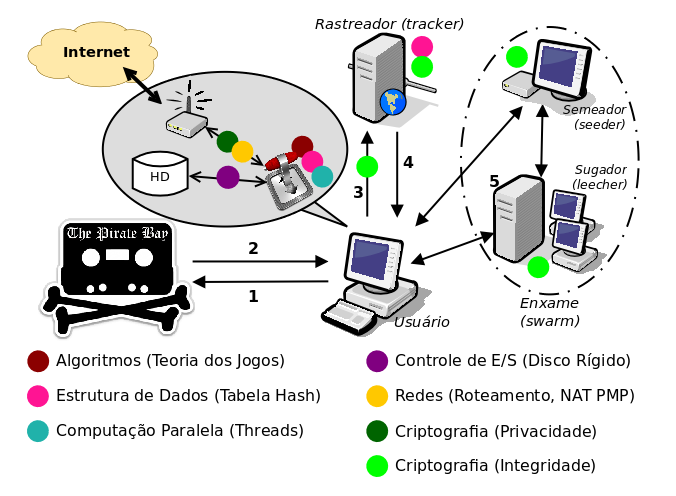
\includegraphics[width=0.64\textwidth]{funcionamento.png}}
        \caption{esquema básico do funcionamento do BitTorrent}
        \label{fig:torrent-basics}
    \end{figure}
\end{comment}

Enquanto um \gls*{peer} estiver fazendo download de um \gls*{torrent}, ele é chamado de
\gls{leecher}, pois ainda consumirá dados de outros \glspl*{peer}; quando o download
acabar, passará a ser um \gls{seeder}, que somente enviará dados.

Os \glspl*{torrentfile} ficam disponíveis em vários sites de índice (às vezes, chamados
de comunidades), como o \href{http://thepiratebay.sx/}{ThePirateBay}, o
\href{http://kickass.to/}{Kickass} ou \href{https://torrentz.eu/}{Torrentz} (muitas
vezes em mais de um deles ao mesmo tempo). Apesar de todo conteúdo compartilhado possuir
um \gls*{torrentfile}, não necessariamente um \gls*{torrentfile} está sendo
compartilhado naquele momento, podendo até mesmo estar extinto.

\Glspl*{peer} que participam do compartilhamento de um \gls*{torrent} específico
fazem parte do \gls{swarm}, onde os dados contidos nesse \gls*{torrent} são
compartilhados por partes com outros \glspl*{peer}.

A quantidade total de partes varia de acordo com cada \gls*{torrent}: o tamanho total
dos arquivos contidos nesse \gls*{torrent} é dividido em blocos de tamanho fixo
(geralmente 256kB) e transmitido de forma independente das outras partes, seguindo uma
ordem estabelecida pelo algoritmo de troca de partes (explicado na seção
~\ref{sec:titfortat}).

Essa ordem varia de acordo com o estado atual do \gls*{swarm} desse \gls*{torrent}.

\newpage
\begin{figure}[H]
    \newlength{\myvsize}
    \newlength{\myhsize}
    \setlength{\myvsize}{5mm}
    \setlength{\myhsize}{0.28\textwidth}

    \centering

    \begin{subfigure}[H]{\myhsize}
        \fbox{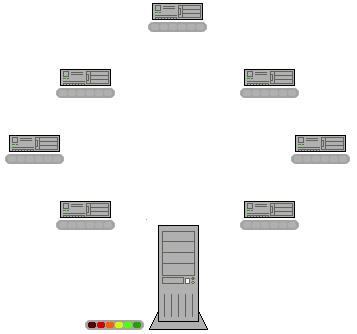
\includegraphics[width=\textwidth]{Torrentcomp_small-0.png}}
        \caption{}
        \label{fig:torrent-repr-0}
    \end{subfigure}%
    \quad %add desired spacing between images (~, \quad, \qquad or blank line)
    \begin{subfigure}[H]{\myhsize}
        \fbox{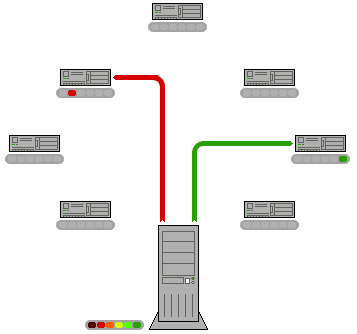
\includegraphics[width=\textwidth]{Torrentcomp_small-1.png}}
        \caption{}
        \label{fig:torrent-repr-1}
    \end{subfigure}%
    \quad
    \begin{subfigure}[H]{\myhsize}
        \fbox{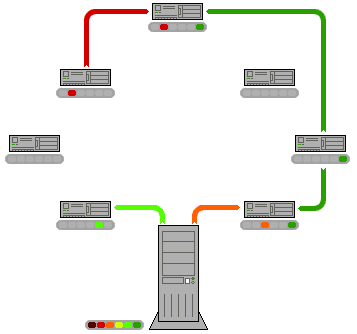
\includegraphics[width=\textwidth]{Torrentcomp_small-2.png}}
        \caption{}
        \label{fig:torrent-repr-2}
    \end{subfigure}

    \vspace{\myvsize}

    \begin{subfigure}[H]{\myhsize}
        \fbox{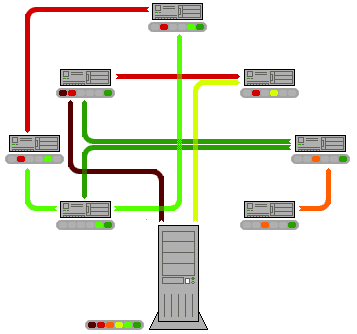
\includegraphics[width=\textwidth]{Torrentcomp_small-3.png}}
        \caption{}
        \label{fig:torrent-repr-3}
    \end{subfigure}%
    \quad
    \begin{subfigure}[H]{\myhsize}
        \fbox{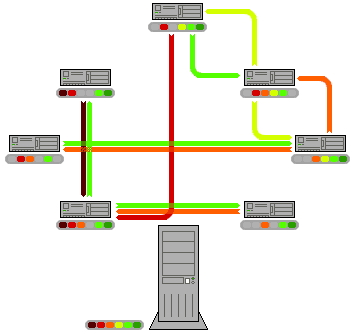
\includegraphics[width=\textwidth]{Torrentcomp_small-4.png}}
        \caption{}
        \label{fig:torrent-repr-4}
    \end{subfigure}%
    \quad
    \begin{subfigure}[H]{\myhsize}
        \fbox{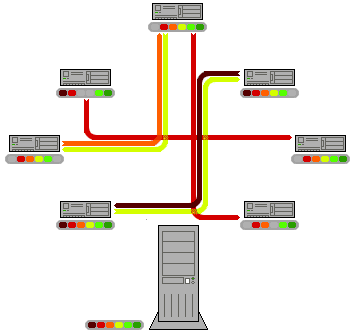
\includegraphics[width=\textwidth]{Torrentcomp_small-5.png}}
        \caption{}
        \label{fig:torrent-repr-5}
    \end{subfigure}

    \vspace{\myvsize}

    \begin{subfigure}[H]{\myhsize}
        \fbox{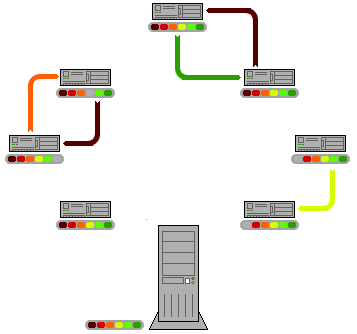
\includegraphics[width=\textwidth]{Torrentcomp_small-6.png}}
        \caption{}
        \label{fig:torrent-repr-6}
    \end{subfigure}%
    \quad
    \begin{subfigure}[H]{\myhsize}
        \fbox{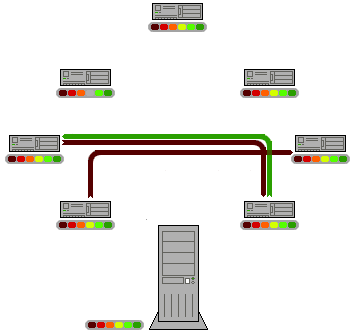
\includegraphics[width=\textwidth]{Torrentcomp_small-7.png}}
        \caption{}
        \label{fig:torrent-repr-7}
    \end{subfigure}%
    \quad
    \begin{subfigure}[H]{\myhsize}
        \fbox{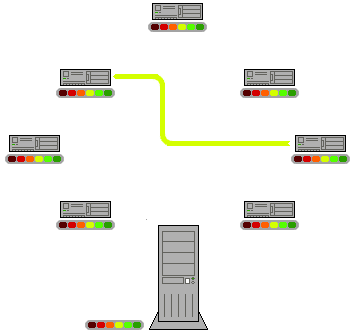
\includegraphics[width=\textwidth]{Torrentcomp_small-8.png}}
        \caption{}
        \label{fig:torrent-repr-8}
    \end{subfigure}

    \vspace{\myvsize}

    \begin{subfigure}[H]{\myhsize}
        \fbox{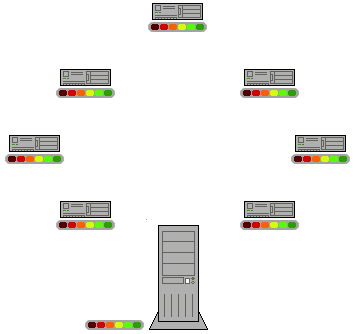
\includegraphics[width=\textwidth]{Torrentcomp_small-9.png}}
        \caption{}
        \label{fig:torrent-repr-9}
    \end{subfigure}

    % TODO: trocar menos (-) por hífen (--)
    \caption{simulação de uma transferência torrent: o seeder, na parte
    inferior das figuras, possui todas as 5 partes de um arquivo, que os outros
    computadores - os leechers - baixam de forma independente e paralela. Fonte:
    \cite{fig:torrent-dl}}
    \label{fig:torrent-repr}
\end{figure}

Todos esses agentes possuem relações múltiplas entre si. Por exemplo, um mesmo
\gls*{torrentfile} pode estar indexado por vários sites indexadores. Como veremos
nos capítulos seguintes, eles contêm uma informação que os identificam unicamente,
gerando consistência entre esses vários sites de busca. Outra observação a ser feita é
que um \gls*{peer} pode estar baixando um ou mais \glspl*{torrent} simultaneamente, ou
seja, participando de vários \glspl*{swarm} ao mesmo tempo. Por fim, em alguns casos,
um mesmo \gls*{torrent} pode possuir uma grande quantidade de \glspl*{peer}
participantes, havendo necessidade de dividí-los em vários \glspl*{swarm}, para fins de
escalabilidade da rede formada.

\begin{figure}[H]
    \centering
    \fbox{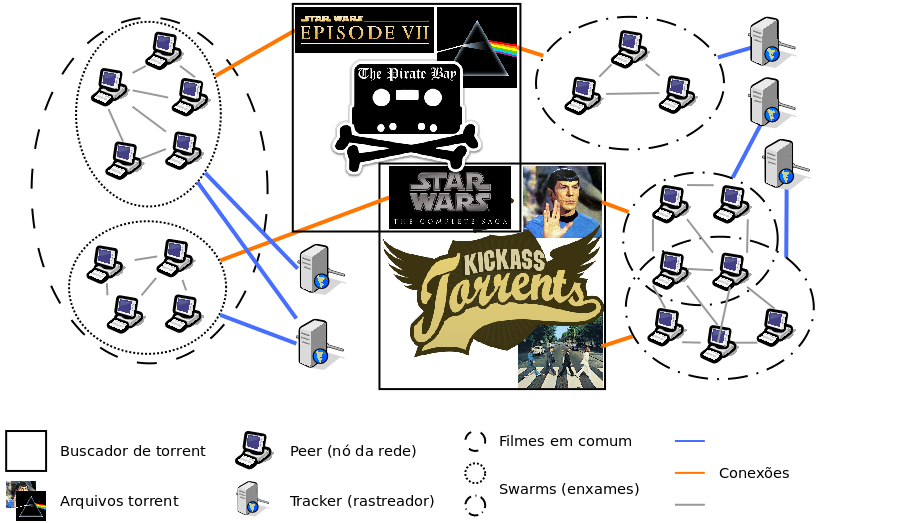
\includegraphics[width=0.85\textwidth]{universobt.png}}
    \caption{amostra de uma rede de conexões BitTorrent}
    \label{fig:torrent-universo}
\end{figure}

\newpage
\subsection*{Arquivo .torrent}

Ao se adicionar um \gls*{torrentfile} em um programa cliente, ocorrem muitas
transmissões de dados antes do download de fato. Para demonstrar isso, usaremos um
\gls*{torrentfile} do filme \enquote{A Noite dos Mortos Vivos}, de 1960
\cite{torrent-file}, que é de domínio público e livre de direitos autorais.

Se abrirmos esse arquivo, veremos uma grande \gls{string}, caracteres diferentes e
incomuns, formando um conteúdo ilegível (na seção binária) e sob uma forma compacta,
mostrado abaixo.

\begin{listing}[H]
    \begin{minted}[
        linenos,
        frame=single,
        numbersep=6pt,
        baselinestretch=1,
        fontfamily=courier,
        gobble=4,
        fontsize=\scriptsize
    ]{text}
    d8:announce36:http://bt1.archive.org:6969/announce13:announce-listll36:http://bt1.
    archive.org:6969/announceel36:http://bt2.archive.org:6969/announceee7:comment13:crea
    tiondatei1343715473e4:infod5:filesld5:crc328:030208fe6:lengthi4127671704e3:md532:627
    f5a428f9e454ccfcb29d31b87169a5:mtime10:10794024804:pathl29:night_of_the_living_dead.
    mpege4:sha140:5e44bb1b3f700240249a5287c64dc02dc56d034bee4:name24:night_of_the_living
    _dead12:piecelengthi4194304e6:pieces23720:<binary>

    (...)

    e6:locale2:en5:title24:night_of_the_living_dead8:url-listl28:http://archive.org/
    download/39:http://ia600301.us.archive.org/22/items39:http://ia700301.us.archive.
    org/22/itemsee
    \end{minted}

    \caption{trecho do conteúdo do arquivo .torrent do filme \enquote{A Noite dos Mortos
    Vivos}, de 1960 \cite{torrent-file}, com a parte binária truncada}
    \label{lst:torrent-file-raw}
\end{listing}

Esse conteúdo está organizado usando a \gls{bencode}, que é uma codificação compacta de
arquivos, especial para \glspl*{torrentfile}, e ininteligível. Com alguma formatação,
podemos enxergar os componentes separadamente, como mostra o código
~\ref{lst:torrent-file-code}.

Esse conteúdo tem significado, sendo utilizado da seguinte forma
\cite{wikitheory:bencoding}:

\begin{itemize}
    \item \textbf{\glspl*{string}} são prefixos de números na base 10, que representam
        comprimentos, seguidos por um caractere \bverb|:| e então o conteúdo. Por
        exemplo, na linha 2, \bverb|8:announce| corresponde à \gls*{string}
        \sverb|"announce"|.

    \item \textbf{números} são representados por um \bverb|i|, seguidos do valor na
        base 10 (sem qualquer limite de tamanho, mas sem zeros precedentes - como em
        \bverb|0003| - e pode ser negativo), terminados por um \bverb|e|. Por exemplo,
        na linha 11, \bverb|i1343715473e| corresponde ao número \sverb|1343715473|.

    \item \textbf{listas} são formadas por \bverb|l|, seguidos por seus elementos
        (também no formato \gls*{bencode}), e então terminados por \bverb|e|. Por
        exemplo, \bverb|l3:foo3:bare| corresponde a \sverb|["foo", "bar"]|. No código
        ~\ref{lst:torrent-file-code}, é presente entre as linhas 43 e 47.

    \item \textbf{dicionários} são definidos por \bverb|d|, seguidos de uma lista
        alternada de chaves e seus valores correspondentes, terminando com \bverb|e|,
        onde as chaves devem estar ordenadas usando-se comparação binária, ao invés da
        usual alfanumérica. Por exemplo, a \gls*{string}
        \bverb|d3:foo3:bar6:foobar6:bazbare| corresponde ao dicionário puro \\
        \sverb|{"foo": "bar", "foobar": "bazbar"}|, e a estrutura mais complexa dada por
        \\ \bverb|d3:fool6:foobar3:bazee| equivale a \sverb|{"foo": ["foobar", "baz"]}|.
\end{itemize}

\begin{listing}[H]
    \begin{minted}[
        linenos,
        frame=single,
        numbersep=6pt,
        baselinestretch=1,
        fontfamily=courier,
        gobble=4,
        fontsize=\scriptsize
    ]{text}
    d
        8:announce
        36:http://bt1.archive.org:6969/announce
        13:announce-list
        l
            l36:http://bt1.archive.org:6969/announcee
            l36:http://bt2.archive.org:6969/announcee
        e
        7:comment
        13:creation date
        i1343715473e
        4:info
        d
            5:files
            l
                d
                    5:crc32
                    8:030208fe
                    6:length
                    i4127671704e
                    3:md5
                    32:627f5a428f9e454ccfcb29d31b87169a
                    5:mtime
                    10:1079402480
                    4:path
                    l29:night_of_the_living_dead.mpege
                    4:sha1
                    40:5e44bb1b3f700240249a5287c64dc02dc56d034b
                e
            e
            4:name
            24:night_of_the_living_dead
            12:piece length
            i4194304e
            6:pieces
            23720:<binary>
        e
        6:locale
        2:en
        5:title
        24:night_of_the_living_dead
        8:url-list
        l
            28:http://archive.org/download/
            39:http://ia600301.us.archive.org/22/items
            39:http://ia700301.us.archive.org/22/items
        e
    e
    \end{minted}
    \caption{trechos formatados de forma legível do conteúdo do arquivo .torrent do
    filme \enquote{A Noite dos Mortos Vivos}, de 1960 \cite{torrent-file}, com a parte
    binária truncada}
    \label{lst:torrent-file-code}
\end{listing}

\subsection*{Magnet Link}

Além do \gls*{torrentfile}, existe uma outra forma de se obter os \glspl*{metadata}
necessários para se iniciar a transmissão, utilizando-se de \glspl{magnetlink}.

\Glspl*{magnetlink}, ao contrário dos \glspl*{torrentfile}, não estão gravados em
algum dispositivo de armazenamento. Basicamente, é um esquema de \gls{uri}, usado
exclusivamente para o protocolo.

No caso citado, o site de origem do \gls*{torrentfile} que estamos usando não fornece um
\gls*{magnetlink} oficialmente. Porém, o Transmission consegue construir uma \gls*{uri}
a partir do arquivo original, para fins de compartilhamento direto. O resultado, após
decodificar o endereço para um formato legível (retirando a \gls{urlencode})
\cite{wiki:urlencode}, foi o seguinte:

\begin{listing}[ht!]
    \begin{minted}[
        linenos,
        frame=single,
        numbersep=6pt,
        baselinestretch=1,
        fontfamily=courier,
        gobble=4,
        fontsize=\scriptsize
    ]{text}
    magnet:?xt=urn:btih:72d7a3179da3de7a76b98f3782c31843e3f818ee
    &dn=night_of_the_living_dead
    &tr=http://bt1.archive.org:6969/announce&tr=http://bt2.archive.org:6969/announce
    &ws=http://archive.org/download/
    &ws=http://ia600301.us.archive.org/22/items/&ws=http://ia700301.us.archive.org/22/items/
    \end{minted}
    \caption{link magnético do arquivo .torrent do filme
    \enquote{A Noite dos Mortos Vivos}, de 1960 \cite{torrent-file}, com parâmetros
    divididos entre linhas para melhor visualização}
    \label{lst:torrent-file-magnet-link}
\end{listing}

Esse endereço é composto por vários pares, compostos por nomes de parâmetros e seus
respectivos valores, sem qualquer ordem específica, formando uma \gls{querystring}.
Podemos dividir esse endereço em partes, cada uma tendo o seu significado:

\begin{itemize}
    \item \textbf{xt}: parâmetro para \emph{exact topic}, ou tópico exato, que contém a
        informação mais importante do \gls*{magnetlink}: o identificador único de
        \glspl*{torrent}. Serve para encontrar e verificar os arquivos especificados.
        No caso, \bverb|urn:btih:<hash>| corresponde ao \gls{urn} \sverb|btih|
        (\emph{BitTorrent Info Hash}), que é a \gls*{string} \gls{hashvalue} resultado
        da \gls{hashfunction} SHA-1, convertida para hexadecimal;

    \item \textbf{dn}: parâmetro que contém o \emph{display name}, ou nome de
        visualização, que é um texto de apresentação amigável para o usuário;

    \item \textbf{tr}: o \emph{address tracker}, ou endereço do \gls*{tracker}, onde o
        programa cliente vai procurar as informações de \glspl*{peer};

    \item \textbf{ws}: endereço do arquivo para \emph{webseed}, ou fornecimento web,
        que é o endereço de Internet de um servidor HTTP ou FTP, que será utilizado como
        alternativa a um \gls*{swarm} problemático \cite{wiki:torrent};
\end{itemize}

\section{Busca por informações}

Quando adicionamos um \gls*{torrent} ao Transmission, o programa salva as
informações em disco durante todo o período em que estas estiverem sendo gerenciadas
por ele. Caso tenha sido por meio de um \gls*{torrentfile}, uma cópia deste é salva em
uma pasta pré-definida para seu controle interno; caso seja por \gls*{magnetlink}, um
novo arquivo é criado contendo as informações obtidas através dele (por questões de
praticidade), para que não necessite fazer essa aquisição dos dados novamente ao ser
aberto, ou quando alguma transferência for pausada e depois continuada.

Após esse arquivamento, o programa processa as informações salvas para deixá-las
carregadas em memória, a fim de obter o \gls*{hashvalue} que identifica o
\gls*{torrentfile}.

\cfile[label="./libtransmission/metainfo.c:367"]{./Codes/chap3/001-leiturametadata.c}

Se aquele arquivo para controle interno tiver sido criado por conta de um
\gls*{magnetlink}, não possuirá a chave \bverb|info| em seu dicionário, mas deverá
conter as chaves \bverb|urn:btih:<hash>| e \bverb|info_hash|.

\cfile[label="./libtransmission/metainfo.c:367"]{./Codes/chap3/002-leiturametadata2.c}

Porém, se o arquivo para controle interno tiver sido criado como cópia do
\gls*{torrentfile}, possuirá o mesmo dicionário, que contém a chave \bverb|info_hash|,
que é utilizada para calcular o \gls*{hashvalue} do arquivo.

\cfile[label="./libtransmission/metainfo.c:367"]{./Codes/chap3/003-leiturametadata3.c}

Outras informações podem ser recuperadas, dependendo da origem do \gls*{torrentfile},
tais como a privacidade do \gls*{torrent}, a lista de arquivos e seus respectivos
tamanhos, \gls*{hashvalue} de cada parte, entre outras. Por fim, termina coletando os
\glspl{announce}.

\cfile[label="./libtransmission/metainfo.c:367"]{./Codes/chap3/004-leiturametadata4.c}

\subsection*{Announce}

Para cada \gls*{swarm} gerenciado, o \gls*{tracker} possui uma lista dos \glspl*{peer}
que participam dele, que é enviada ao \gls*{peer} que a requer por meio de uma
\gls{httpget}. Quando essa requisição é recebida pelo \gls*{tracker}, este incluirá ou
atualizará um registro para o \gls*{peer} solicitante, e devolverá uma lista de 50
\glspl*{peer} aleatórios, de forma uniforme, que fazem parte do \gls*{swarm}. Não
havendo essa quantidade total, a lista toda será enviada ao requisitante. Caso
contrário, a aleatoriedade proporcionará uma diversidade de listas enviadas,
ocasionando robustez ao sistema \cite{wikitheory:tracker-response}.

Esse contato entre um \gls*{peer} e um \gls*{tracker} é chamado de \gls{announce}, que
pode ser feito usando-se tanto o \gls{tcp}, bem como o \gls{udp}, e é como \glspl*{peer}
podem passar várias informações, usando um dicionário no formato \gls*{bencode}:

\begin{itemize}
    \item \textbf{info\_hash}: \gls*{hashvalue} de 20 bytes resultante da
    \gls*{hashfunction} SHA-1, com \gls*{urlencode}, do valor da chave \bverb|info| do
    arquivo \gls*{torrentfile};

    \item \textbf{peer\_id}: \gls*{string} de 20 bytes, com \gls*{urlencode}, usado como
    identificador único do programa cliente, gerado no ínício da sua execução. Para
    isso, provavelmente deverá incorporar informações do computador, a fim de se gerar
    um valor único;

    \item \textbf{uploaded}: a quantidade total de dados, em bytes, enviados desde o
    momento em que o cliente enviou o primeiro aviso ao \gls*{tracker};

    \item \textbf{downloaded}: a quantidade total de dados, em bytes, recebidos desde
    momento em que o cliente enviou o primeiro aviso ao \gls*{tracker};

    \item \textbf{left}: a quantidade total de dados, em bytes, que faltam para o
    requisitante terminar o download do \gls*{torrent} e passe a ser um \gls*{seeder};

    \item \textbf{compact} (opcional): se o valor passado for 1, significa que o
    requisitante aceita respostas compactas. A lista de \glspl*{peer} enviada é
    substituída por uma única \gls*{string} de peers, sendo que cada \gls*{peer} terá
    6 bytes, onde os 4 bytes iniciais são o host e os 2 bytes finais são a porta de
    transmissão. Por exemplo, o endereço IP 10.10.10.5:80 seria transmitido como
    \bverb|0A 0A 0A 05 00 80|. Deve-se observar que alguns \glspl*{tracker} suportam
    somente conexões deste tipo para otimização da utilização da banda de rede e, para
    isso, ou recusarão requisições sem \bverb|compact=1| ou, caso não as recusem,
    enviarão respostas compactas a menos que a requisição possua \bverb|compact=0|;

    \item \textbf{no\_peer\_id} (opcional): sinaliza que o \gls*{tracker} pode omitir o
    campo \textcolor{Bittersweet}{\texttt{peer\_id}} no dicionário de \glspl*{peer},
    porém será ignorado caso o modo compacto esteja habilitado;

    \item \textbf{event} (opcional): pode possuir os valores \sverb|started|
    (iniciado), \sverb|completed| (terminado), \sverb|stopped| (parado), ou vazio para
    não especificar.

    \begin{itemize}
        \item \emph{started} : a primeira requisição para o \gls*{tracker} deve enviar
        este valor;
        \item \emph{stopped} : avisa que o programa cliente está fechando;
        \item \emph{completed} : quando o download que estava ocorrendo termina numa
        mesma execução do programa cliente (não é enviado quando o programa cliente é
        iniciado com o \gls*{torrent} em 100\%);
    \end{itemize}

    \item \textbf{port} (opcional): o número da porta de conexão que o programa cliente
    está escutando por transmissões de dados. Em geral, portas reservadas para
    BitTorrent estão entre 6881 e 6889. Se esse for o caso, pode ser omitido;

    \item \textbf{ip} (opcional): o endereço IP verdadeiro do requisitante, no formato
    legível do IPv4 (4 conjuntos de número de 0 a 255 separados por \bverb|.|) ou do
    IPv6 (8 conjuntos de números hexadecimais de 4 dígitos separados por \bverb|:|).
    Não é sempre necessário, pois o endereço pode ser conhecido através da requisição.
    Assim, é usado quando o programa cliente está se comunicando com o \gls*{tracker}
    através de um \gls{proxy} ou quando ambos (cliente e \gls*{tracker}) estão no mesmo
    lado local de um roteador - com \gls{nat} -, pois, nesse caso o endereço IP não é
    roteável;

    \item \textbf{numwant} (opcional): quantidade de \glspl*{peer} que o requisitante
    gostaria de receber do \gls*{tracker}. É permitido valor zero. Se omitido, assumirá
    valor padrão de 50;

    \item \textbf{key} (opcional): mecanismo de identificação adicional para o programa
    cliente provar sua identidade, caso tenha ocorrido mudança no seu endereço IP;

    \item \textbf{trackerid} (opcional): se a resposta de um \gls*{announce} anterior
    continha o endereço IP de um \gls*{tracker}, deve ser enviado neste campo;
\end{itemize}

%\newpage
\cfile[label="./libtransmission/announcer-common.h:127"]{./Codes/chap3/005-announcestruct.c}
\cfile[label="./libtransmission/announcer.c:1200"]{./Codes/chap3/006-announce.c}

Como resposta, é recebida um outro dicionário em \gls*{bencode}, podendo conter as
seguintes chaves:

\begin{itemize}
    \item \textbf{failure\_reason}: se presente, não podem existir outras chaves no
    dicionário. Seu valor é uma \gls*{string} de mensagem de erro legível sobre o
    porque a requisição falhou;

    \item \textbf{warning\_message} (opcional): similar à chave
    \bverb|failure\_reason|, mas com a requisição tendo sido processada normalmente. A
    mensagem é mostrada como um erro;

    \item \textbf{interval}: intervalo, em segundos, que o cliente deve esperar emtre
    requisições de \gls*{announce} ao \gls*{tracker};

    \item \textbf{min\_interval} (opcional): intervalo mínimo, em segundos, entre
    requisições de \gls*{announce}. Se presente, o pragrama cliente não deve efetuar
    essas requisições acima da frequência estipulada;

    \item \textbf{tracker\_id}: \gls*{string} que o programa cliente deve enviar de
    volta nas próximas requisições. Se ausente e um valor tiver sido passado
    anteriormente, o uso desse valor antigo é continuado;

    \item \textbf{complete}: quantidade de \glspl*{seeder};

    \item \textbf{incomplete}: quantidade de \glspl*{leecher};

    \item \textbf{peers}: pode ser uma das opções

    \begin{enumerate}
        \item lista de dicionários \gls*{bencode}, com as seguintes chaves:

        \begin{itemize}
            \item \textbf{peer\_id}: identificador de um \gls*{peer} na forma de
            \gls*{string}, escolhido por si próprio da mesma forma que a descrito pela
            definição de requisição;

            \item \textbf{ip}: endereço IP do \gls*{peer} nos formatos IPv4 (4 octetos)
            ou IPv6 (valores hexadecimais), ou ainda o nome de domínio DNS (string);

            \item \textbf{port}: número da porta utilizada pelo \gls*{peer};
        \end{itemize}

        \item \gls*{string} binária cujo tamanho é de 6 bytes para cada \gls*{peer},
        onde os 4 primeiros representam o endereço IP e os 2 últimos são o número da
        porta, em notação de rede (\emph{big endian});
    \end{enumerate}
\end{itemize}

\begin{listing}[H]
    \begin{minted}[
        linenos,
        frame=single,
        numbersep=6pt,
        baselinestretch=1,
        fontfamily=courier,
        gobble=4,
        fontsize=\scriptsize
    ]{text}
    * About to connect() to exodus.desync.com port 6969 (#8)
    *   Trying 208.83.20.164...
    *
    * Connected to exodus.desync.com (208.83.20.164) port 6969 (#8)
    > GET /announce?info_hash=\%88\%15\%8c\%7bW\%e0\%85\%21\%86~\%d0\%b5\%de\%06\%5b\%
    7dWI\%cf\%d7&peer_id=-TR2820-ne1joqgh8z9o&port=51413&uploaded=0&downloaded=0&left=52
    406288292&numwant=80&key=6ee99240&compact=1&supportcrypto=1&requirecrypto=1&event=
    started HTTP/1.1
    User-Agent: Transmission/2.82
    Host: exodus.desync.com:6969
    Accept: */*
    Accept-Encoding: gzip;q=1.0, deflate, identity

    < HTTP/1.1 200 OK
    < Content-Type: text/plain
    < Content-Length: 136
    <
    * Connection #8 to host exodus.desync.com left intact
    Announce response:
    < {
        "complete": 1,
        "downloaded": 11,
        "incomplete": 6,
        "interval": 1732,
        "min interval": 866,
        "peers": \"<binary>\"
    }
    \end{minted}

    \caption{Logs do Transmission sobre uma requisição de announce e a respectiva
    resposta, com o conteúdo binário truncado}
    \label{lst:announce}
\end{listing}

Essa comunicação ocorre nas seguintes situações:

\begin{itemize}
    \item no primeiro contato do \gls*{peer}, para que ele tenha acesso a um
        \gls*{swarm};

    \item a cada período de tempo, estipulado pelo tracker, para que o \gls*{peer}
        continue mostrando que ainda está conectado, além de poder receber endereços de
        \glspl*{peer} novos;

    \item quando a quantidade de \glspl*{peer} conhecidos que estiverem ativos for
        menor do que 5;

    \item quando terminar o download, notificando que passou a ser um \gls*{seeder};

    \item quando sair do \gls*{swarm}, seja por desconexão ou por encerramento do
        programa cliente;
\end{itemize}

\subsection*{Scrape}

Além do \gls*{announce}, outra forma de troca de informação entre \glspl*{peer} e
\glspl*{tracker} se dá pelo \gls{scrape}. Geralmente usado pelos programas cliente para
decidir quando realizar um \gls*{announce}, informa o número de \glspl*{peer},
\glspl*{leecher} e \glspl*{seeder} de uma lista de um ou mais \glspl*{torrent}. É dessa
forma que os sites de indexação sabem dessas informações e as apresentam nas em páginas.

A requisição de \gls*{scrape} pode ser sobre todos os \glspl*{torrent} que o
\gls*{tracker} gerencia ou sobre um ou mais \glspl*{torrent} em específico, quando são
passados seus respectivos \glspl*{hashvalue}. Sua resposta é um dicionário na forma
\gls*{bencode} contendo as chaves

\begin{itemize}
    \item \textbf{files}: um dicionário contendo um par chave-valor para cada
    \gls*{torrent} especificado na requisição do \gls*{scrape} através do
    \gls*{hashvalue} do \gls*{torrent} de 20 bytes:

    \begin{itemize}
        \item \textbf{complete}: quantidade de \glspl*{seeder};

        \item \textbf{incomplete}: quantidade de \glspl*{leecher};

        \item \textbf{downloaded}: quantidade total de vezes que o \gls*{tracker}
        registrou uma finalização (\sverb|event=complete| ao término de um download);

        \item \textbf{name} (opcional): o nome interno do \gls*{torrent}, como
        especificado pelo respectivo \gls*{torrentfile}, na sua seção \bverb|info|;
    \end{itemize}
\end{itemize}

Da mesma forma que o \gls*{announce}, o \gls*{scrape} é um endereço do \gls*{tracker}
usando-se o \gls*{tcp} ou o \gls*{udp}, e é tratado de forma semelhante pelo
Transmission.

\cfile[label="./libtransmission/announcer-common.h:37"]{./Codes/chap3/007-scrapestruct.c}
\cfile[label="./libtransmission/announcer.c:1397"]{./Codes/chap3/008-scrape.c}

\begin{listing}[H]
    \begin{minted}[
        linenos,
        frame=single,
        numbersep=6pt,
        baselinestretch=1,
        fontfamily=courier,
        gobble=4,
        fontsize=\scriptsize
    ]{text}
    * About to connect() to www.mvgroup.org port 2710 (#1)
    *   Trying 88.129.153.50...
    * Connected to www.mvgroup.org (88.129.153.50) port 2710 (#1)
    > GET /scrape?info_hash=\%83F\%24\%b62\%e5Q\%cc4\%10h\%ba\%1e8\%e2C\%f7\%80\%01\%87 HTTP/1.1
    User-Agent: Transmission/2.82
    Host: www.mvgroup.org:2710
    Accept: */*
    Accept-Encoding: gzip;q=1.0, deflate, identity

    * HTTP 1.0, assume close after body
    < HTTP/1.0 200 OK
    <
    * Closing connection 1
    Scrape response:
    < {
        "files": {
            \"<binary>\": {
                "complete": 9,
                "downloaded": 59074,
                "incomplete": 2
            }
        }
    }
    \end{minted}

    \caption{Logs do Transmission sobre uma requisição de scrape e a respectiva
    resposta, com o conteúdo binário truncado}
    \label{lst:scrape}
\end{listing}

\subsection*{Convenção de scrape de trackers}

O endereço de \gls*{scrape} pode ser obtido a partir do endereço de \gls*{announce},
seguindo-se a seguinte convenção:

\begin{enumerate}
    \item comece a partir do endereço de \gls*{announce}

    \item encontre o último caractere \bverb|/|

    \item se o texto que segue a última \bverb|/| não for \sverb|announce|, é um sinal
    que o \gls*{tracker} não segue a convenção

    \item caso contrário, substituir \sverb|announce| por \sverb|scrape|
\end{enumerate}

Alguns exemplos:

\begin{itemize}
    \item suportam \sverb|scrape|
        \begin{enumerate}
            \item \url{http://example.com/announce} $\rightarrow$ \url{http://example.com/scrape}
            \item \url{http://example.com/announce.php} $\rightarrow$ \url{http://example.com/scrape.php}
            \item \url{http://example.com/x/announce} $\rightarrow$ \url{http://example.com/x/scrape}
            \item \url{http://example.com/announce?x2\%0644} $\rightarrow$ \url{http://example.com/scrape?x2\%0644}
        \end{enumerate}

    \item não suportam \sverb|scrape|
        \begin{enumerate}
            \item \url{http://example.com/a}
            \item \url{http://example.com/announce?x=2/4}
            \item \url{http://example.com/x\%064announce}
        \end{enumerate}
\end{enumerate}

%\section{Fontes de arquivos}

Com a requisição do \gls*{announce}, o Transmission recebe a sua resposta e prepara
esses dados para utilização, carregando-os em memória.

\cfile[label="./libtransmission/announcer-http.c:288"]{./Codes/chap3/009-httpannounce.c}
\cfile[label="./libtransmission/announcer-http.c:189"]{./Codes/chap3/010-onhttpannouncedone.c}

Após essa preparação dos dados da resposta do \gls*{announce}, cuja informação
principal é a lista de \glspl*{peer}, o Transmission gerencia o tempo para a próxima
requisição periódica de \gls*{announce} ou \gls*{scrape}. Além disso, sinaliza para a
\gls{thread} principal do programa que recebeu a resposta do \gls*{tracker}.

\cfile[label="./libtransmission/announcer.c:1012"]{./Codes/chap3/011-onannouncedone.c}
\cfile[label="./libtransmission/announcer.c:523"]{./Codes/chap3/012-publicapeers.c}

A \gls*{thread} principal percebe que foi sinalizado o recebimento de uma resposta de
\gls*{tracker} e começa a utilizar a lista de \glspl*{peer} adquirida, adicionando-os ao
\gls{pool} do objeto em memória que representa o \gls{swarm}.

\cfile[label="./libtransmission/torrent.c:552"]{./Codes/chap3/013-ontrackerresponse.c}
\cfile[label="./libtransmission/peer-mgr.c:2113"]{./Codes/chap3/014-addpex.c}

Essa inclusão é condicionada ao fato de que o endereço de um \gls*{peer} ainda não está
contido na lista de \glspl*{peer}.

\cfile[label="./libtransmission/peer-mgr.c:1852"]{./Codes/chap3/015-verificapeer.c}

Assim, a lista de \glspl*{peer} do Transmission está pronta para ser utilizada nos
pedidos das partes do \gls*{torrent}.

\newpage
\section{Tabelas Hash Distribuídas e o Kademlia}

Os \glspl{dht} surgiram quando buscas em \glspl{p2p} não eram eficientes, fosse pelos
problemas da supercentralização dos sistemas ou pela falta dela, tentando criar uma
maneira híbrida de buscar e localizar recursos nessas redes.

Existem duas formas de se encontrar objetos: busca e endereçamento. A primeira se baseia
no casamento de palavras-chave com as das descrições dos objetos, sendo mais amigável
para um usuário pois não necessita de formas complexas de identificação. Porém, é mais
difícil de se tornar eficiente, além de precisar conferir também os objetos para saber
se são o mesmo. As \glspl*{p2p} descentralizadas utilizavam desta abordagem.

A segunda, no entanto, utiliza endereços que possam identificá-los de forma única. Dessa
forma, um objeto é exclusivamente identificável, sendo possível encontrá-lo
eficientemente. Contudo, é necessário algum procedimento de se conhecer seu nome único,
além de ser requerido manter uma estrutura organizada por endereços. Historicamente, as
\glspl*{p2p} de estrutura centralizada se baseavam neste método.

Uma outra maneira de organizar esses objetos através da rede é de organizar as conexões
entre os diversos \glspl*{peer}, que acabam formando redes superpostas (\emph{overlay
networks}), que são redes virtuais que figuram sobre as tradicionais redes IP.

Anteriormente ao BitTorrent, nas \glspl*{p2p} de estrutura centralizada, o servidor
central tentava conhecer a situação de cada um dos \glspl*{peer} da rede, enviando
mensagens diretamente a eles. Gerenciar muitos \glspl*{peer} ao mesmo tempo
sobrecarregava o \emph{hardware} do servidor, ou forçava o seu desligamento. Por outro
lado, quando a rede tinha estrutura descentralizada, ocorria o fenômeno chamado de
inundação de mensagens, no qual estas eram repassadas entre \glspl*{peer}
intermediários até o \gls*{peer} de destino. Esse repasse excessivo acarretava
sobrecarga de processamento (\emph{overhead}) dos intermediários, além de gerar
mensagens falso-negativas.

Assim, as \glspl*{p2p} necessitam de funcionalidades eficientes para que um \gls*{peer}
possa entrar e sair do \emph{overlay}, assim como armazenar objetos e encontrá-los
(usando endereçamento). Tal eficiência é conseguida através de \glspl{dht}, onde todas
essas funcionalidades dependem da troca de mensagens eficiente entre \glspl*{peer}.

\begin{figure}[H]
    \centering
    \fbox{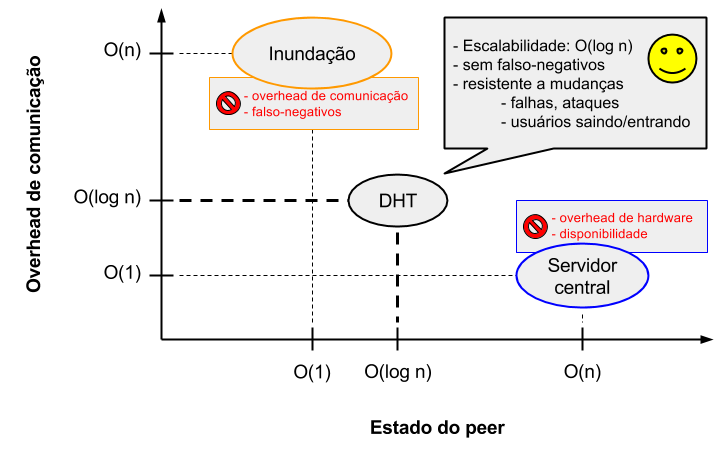
\includegraphics[width=0.85\textwidth]{graph-dht.png}}
    %\caption{amostra de uma rede de conexões BitTorrent}
    %\label{fig:torrent-universo}
\end{figure}

A funcionalidade do \gls*{dht} passou anos sendo utilizado extraoficialmente à
especificação do protocolo, quando, enfim, foi adicionada em 2008
\cite{site:bittorrent-dht}.

\subsection*{Kademlia}

O Kademlia é um \gls*{dht} criado em 2002 \cite{artigo:kademlia} com o objetivo de
melhorar os métodos de busca atuais (Napster e\gls*{gnutella}), que eram ineficientes.
Assim como os outros algoritmos de \gls*{dht}, ele se baseou na estrutura informalmente
conhecida como \enquote{rede de Plaxton} (\emph{Plaxton mesh}), nome que remete a um
dos seus autores \cite{artigo:dht}. Por ter causado boas impressões, foi usado na
implementação da busca de arquivos no programa cliente eMule.

O algoritmo implementa uma rede \emph{overlay} cuja estrutura e comunicação se baseiam
na procura de seus nós. Cada um destes nós é identificado por um identificador único
(ID), que serve tanto para a identificação quanto para a localização de valores na
\gls*{hashtable}. Durante uma busca, o processo deve conhecer a chave (que é um
\gls*{hashvalue}) associado ao objeto - neste caso, o ID do \gls*{torrent}, que é seu
\gls*{hashvalue} - e explora a rede em passos, encontrando nós mais próximos da chave,
até encontrar o valor buscado ou não nós existirem mais próximos que o atual. Dessa
forma, para uma rede com $n$ nós, o algoritmo visita apenas $O(\log n)$ nós.

\subsection*{Funcionamento}

No Kademlia, objetos e nós possuem IDs únicos de 160 bits: enquanto o primeiro utiliza
o \gls*{hashvalue} de 20 bytes SHA-1 da chave \bverb|info_hash| do \gls*{torrentfile},
o segundo é um valor aleatório escolhido pelo próprio programa.

Como este \gls*{dht} é construído com base em distâncias entre nós, a função de medida
escolhida foi

\begin{equation}
    d(x,y) = x \oplus y
\end{equation}

pois possui algumas propriedades em comum com a equação de distância euclidiana usual.
Assim, seguem suas propriedades:

\begin{itemize}
    \item $d(x,x) = 0$
    \item $x \neq y$, $d(x,y) > 0$
    \item simetria: $\forall x,y$, $d(x,y) = d(y,x)$
    \item desigualdade triangular: $d(x,y) + d(y,z) \geq d(x,z)$. \\
        Isto vem do fato de $d(x,z) = d(x,y) \oplus d(y,z)$ e que $\forall a \geq 0,
        \forall b \geq 0 : a + b \geq a \oplus b$
    \item unidirecionalidade: para um dado ponto $x$ e uma distância $\Delta > 0$,
        existe exatamente um ponto $y$ tal que $d(x,y) = \Delta$. Isso garante que todas
        as procuras por uma mesma chave convirjam para um mesmo percurso, independente
        do ponto de partida.
\end{itemize}

\subsubsection*{Estado dos nós}

Cada nó do Kademlia armazena informações sobre outros nós para rotear mensagens de
pesquisa. Para cada bit $i$ dos IDs (cada ID tem 160 bits) é mantido um \gls{kbucket},
que contém os nós cuja distância até ele está entre $2^i$ e $2^{i+1}$. Esses
\glspl*{kbucket} são listas de endereço IP, porta de comunicação \gls*{udp} e ID de
nós, ordenadas pelo horário da última notícia destes. Para distâncias pequenas, essas
listas geralmente serão vazias, enquanto para distâncias maiores poderão ser de tamanho
$k$. Este valor, que é o de replicação do sistema, é escolhido de tal forma que esses
$k$ nós possuam grande probabilidade de não falharem na próxima hora.

Quando um nó \textbf{A} recebe uma mensagem de outro nó \textbf{B}, o \gls*{bucket}
correspondente ao ID do remetente (nó \textbf{B}) é atualizado. Disto, podem ocorrer as
seguintes situações:

\newpage
\begin{itemize}
    \item \textbf{B} já existe no \gls*{bucket}: passa a ser o primeiro da lista, pois
        existiu mensagem recente.

    \item \textbf{B} não existe no \gls*{bucket}:
        \begin{itemize}
            \item \gls*{bucket} não está cheio: \textbf{B} é adicionado no começo da
                lista.
            \item \gls*{bucket} cheio: é enviado um \emph{ping} para o nó do final da
                lista (nó \textbf{C}), contatado há mais tempo

            \begin{itemize}
                \item \textbf{C} não responde ao \emph{ping}: \textbf{C} é retirado da
                lista e \textbf{B} é inserido no início
                \item \textbf{C} responde ao \emph{ping}: \textbf{C} é movido para o
                início da lista e \textbf{B} é ignorado
            \end{itemize}
        \end{itemize}

\end{itemize}

Por conta disso, ocorre que nós mais antigos e funcionais são preferidos, pois quanto
mais tempo um nó está conectado, mais provável ele se manterá conectado por mais 1 hora
\cite{artigo:gnutella-uptime}. Outra vantagem disso é a resistência a alguns ataques de
negação de serviço, pois mesmo que ocorra uma inundação de novos nós, estes só seriam
inseridos nos \glspl*{kbucket} se os antigos fossem excluídos.

\subsubsection*{Protocolo}

O protocolo de mensagens \gls*{dht} utiliza o formato KRPC, que é um mecanismo de
chamada \gls{rpc} que envia dicionários \gls*{bencode} através de \gls*{udp}, uma única
vez por chamada (um pacote para a requisição, outro para a resposta), sem novas
tentativas.

Existem 3 tipos de mensagem: consulta (\emph{query}), resposta (\emph{response}) e erro
(\emph{error}). Para o protocolo \gls*{dht}, são 4 comandos \emph{query}: \bverb|ping|,
\bverb|find_node|, \bverb|get_peers| e \bverb|announce_peer|. Em todos, o nó sempre
enviará seu ID como valor da chave \bverb|id|.

Uma mensagem KRPC é um dicionário com 2 chaves comuns a todos os 4 comandos: \bverb|y|,
que especifica o tipo da mensagem, e \bverb|t|, que corresponde ao ID da transação.
Este é um número binário convertido para \gls*{string}, geralmente formada por 2
caracteres, possuindo valor até $2^{16}$, e devolvida nas respostas. Isso permite que
estas se relacionem a múltiplas consultas a um nó.

Cada tipo de mensagem possui formatos diferentes entre si, permitindo parâmetros
adicionais para cada chamada, possuindo as seguintes chaves e seus respectivos valores:

\newpage
\begin{itemize}
    \item \emph{query}
        \begin{itemize}
            \item \bverb|y|: caractere \sverb|q|
            \item \bverb|q|: string do comando desejado (\sverb|ping|,
                \sverb|find_node|, \sverb|get_peers|, \sverb|announce_peer|)
            \item \bverb|a|: dicionário contendo parâmetros adicionais, dependendo do
                comando passado na chave \bverb|q|
        \end{itemize}

    \item \emph{response}
        \begin{itemize}
            \item \bverb|y|: caractere \sverb|r|
            \item \bverb|r|: dicionário contendo valores da resposta, dependendo do
                comando passado na chave \bverb|q|
        \end{itemize}

    \item \emph{error}
        \begin{itemize}
            \item \bverb|y|: caractere \sverb|e|

            \item \bverb|e|: lista contendo 2 elementos: código (número inteiro) e
                mensagem para o erro (\gls*{string}). Os erros podem ser:
                \begin{itemize}
                    \item 201 (Generic Error): erros genéricos
                    \item 202 (Server Error): erros de servidor
                    \item 203 (Protocol Error): para pacote mal formado, argumento
                        inválido ou token incorreto
                    \item 204 (Method Unknown): comando não conhecido
                \end{itemize}

            \item exemplo: \\
                \bverb|d1:eli201e23:A Generic Error Ocurrede1:t2:aa1:y1:ee|
                (\gls*{bencode}) \\
                \sverb|{"t":"aa", "y":"e", "e":[201, "A Generic Error Ocurred"]}|
                (\gls*{string})
        \end{itemize}
\end{itemize}

As informações retornadas podem ser sobre \glspl*{peers} ou nós \gls{dht}: enquanto o
primeiro é a \enquote{informação compacta de endereço IP/porta} - string de 6 bytes (4
bytes iniciais para o endereço IP e 2 bytes finais para a porta de comunicação usada)
-, o segundo é a \enquote{informação compacta de nó} - string de 26 bytes (20 bytes
iniciais para o ID do nó e 6 bytes finais para a respectiva informação compacta de
endereço IP/porta).

\subsubsection*{Comandos}

Os 4 comandos de \emph{query} do \gls*{dht} (\bverb|ping|, \bverb|find_node|,
\bverb|get_peers| e \bverb|announce_peer|) estão definidos da seguinte forma.

% \newpage
\subsubsubsection{ping}

É o comando mais simples, que verifica se o nó está online. Possui um único argumento,
que é uma chave \bverb|id|, que é o ID do nó consultante (na requisição) ou do nó
consultado (na resposta).

\begin{itemize}
    \item requisição \\
        \bverb|d1:ad2:id20:abcdefghij0123456789e1:q4:ping1:t2:aa1:y1:qe|
        (\gls*{bencode}) \\
        \sverb|{"t":"aa", "y":"q", "q":"ping", "a":{"id":"abcdefghij0123456789"}}|
        (\gls*{string})

    \item resposta \\
        \bverb|d1:rd2:id20:mnopqrstuvwxyz123456e1:t2:aa1:y1:re|
        (\gls*{bencode}) \\
        \sverb|{"t":"aa", "y":"r", "r": {"id":"mnopqrstuvwxyz123456"}}|
        (\gls*{string})
\end{itemize}

\cfile[label="./third-party/dht/dht.c:2291"]{./Codes/chap3/016-dht-macros.c}
\cfile[label="./third-party/dht/dht.c:2341"]{./Codes/chap3/017-dht-ping.c}

\newpage
\subsubsubsection{find\_node}

Este comando é usado para encontrar as informações do nó dado seu ID. Necessita enviar 2
argumentos: a chave \bverb|id| e o ID do nó consultante, e a chave \bverb|target| e o ID
do nó cujas informações o consultante está procurando (ou nó alvo). O nó consultado
deve responder com a chave \bverb|nodes| contendo uma \gls*{string} com a informação
compacta do nó alvo ou dos $k$ nós bons (que fizeram contato recentemente) mais
próximos que estão contidos em sua tabela de roteamento, de 1 ou mais \glspl*{kbucket}.

No artigo do Kademlia \cite{artigo:kademlia}, os autores explicam o funcionamento do
algoritmo da busca:

\blockquote{O procedimento mais importante que um participante do Kademlia deve realizar
é encontrar os $k$ nós próximos a um dado ID de nó. Nós chamamos esse procedimento de
\emph{busca por nós}. Kademlia utiliza de um algoritmo recursivo nas buscas por nós. O
disparador das buscas começa escolhendo $\alpha$ nós do \gls*{bucket} não-vazio mais
próximo (ou, se esse \gls*{bucket} tiver menos que $\alpha$ entradas, utiliza desses
$\alpha$ nós mais próximos que conhece). Então, o disparador envia chamadas \gls*{rpc}
assíncronas paralelas de comandos \textbf{find\_node} para esses $\alpha$ nós
escolhidos. $\alpha$ é um parâmetro de concorrência geral ao sistema, assumindo valor
como 3.

No passo recursivo, o disparador reenvia chamadas a \textbf{find\_node} para os nós que
conheceu das chamadas \gls*{rpc} passadas. (Esta recursão pode começar antes que todos
os $\alpha$ nós anteriores tenham respondido). Dos $k$ nós que o disparador concluiu
serem mais próximos ao alvo, ele pega $\alpha$ que ainda não foram consultados e envia
chamadas \gls*{rpc} \textbf{find\_node}. Nós que falharem em responder rapidamente são
desconsiderados até que respondam. Se uma rodada de comandos \textbf{find\_node} não
retornar algum nó mais próximo do que os nós já conhecidos, o disparador reenvia
comandos \textbf{find\_node} para todos os $k$ nós mais próximos que ainda não foram
consultados. A busca termina quando o disparador tiver consultado e obtido respostas de
todos os $k$ nós mais próximos conhecidos.}

Porém, o Transmission implementa essa busca de forma mais flexível e simples. De início,
busca o \gls*{bucket} no qual o ID procurado está ou que contém nós mais próximos.

\cfile[label="./third-party/dht/dht.c:2536"]{./Codes/chap3/020-dht-findclosestnodes.c}

A busca do \gls*{bucket} itera sobre a lista ligada de \glspl*{bucket}.

\cfile[label="./third-party/dht/dht.c:129"]{./Codes/chap3/018-dht-structs.c}
\cfile[label="./third-party/dht/dht.c:464"]{./Codes/chap3/019-dht-findbucket.c}

Caso retorne o \gls*{bucket} mais provável, efetua buscas internas nele. Se ele possuir
elementos vizinhos anteriores ou posteriores, também busca por nós neles.

\cfile[label="./third-party/dht/dht.c:2523"]{./Codes/chap3/021-dht-bufferclosestnodes.c}
\cfile[label="./third-party/dht/dht.c:2476"]{./Codes/chap3/022-dht-insertclosestnode.c}

Ao fim da busca, envia a lista de nós que encontrou como resposta à mensagem de
\bverb|find_node| recebida.

\begin{comment}
When a node wants to find peers for a torrent, it uses the distance metric to compare
the infohash of the torrent with the IDs of the nodes in its own routing table. It then
contacts the nodes it knows about with IDs closest to the infohash and asks them for the
contact information of peers currently downloading the torrent. If a contacted node
knows about peers for the torrent, the peer contact information is returned with the
response. Otherwise, the contacted node must respond with the contact information of
the nodes in its routing table that are closest to the infohash of the torrent. The
original node iteratively queries nodes that are closer to the target infohash until it
cannot find any closer nodes. After the search is exhausted, the client then inserts
the peer contact information for itself onto the responding nodes with IDs closest to
the infohash of the torrent.

The return value for a query for peers includes an opaque value known as the "token."
For a node to announce that its controlling peer is downloading a torrent, it must
present the token received from the same queried node in a recent query for peers. When
a node attempts to "announce" a torrent, the queried node checks the token against the
querying node's IP address. This is to prevent malicious hosts from signing up other
hosts for torrents. Since the token is merely returned by the querying node to the same
node it received the token from, the implementation is not defined. Tokens must be
accepted for a reasonable amount of time after they have been distributed. The
BitTorrent implementation uses the SHA1 hash of the IP address concatenated onto a
secret that changes every five minutes and tokens up to ten minutes old are accepted.
\end{comment}

\section{Peer Exchange}

\todo[inline]{Funciona somente no \gls*{swarm}!}

\todo[inline]{Explicar a funcionalidade de PEX}

\section{Jogo da troca de arquivos}
\label{sec:titfortat}

Explicarei o algoritmo tit-for-tat padrão do protocolo BitTorrent, que vem da Teoria
dos Jogos, e como o Transmission o implementa.

\afterpage{\clearpage}